\iffalse
\title{Assignment}
\author{EE24BTECH11038}
\section{xe}
\chapter{2016}
\fi
\item Consider the following figures shown below. The objects are marked as A1, A2, B1, B2 and C1, C2 and the flow directions over these objects are shown by the respective arrow placed to the left of the object. Freestream velocities are same for all the cases. Amongst these objects, A1, A2, B1 and C1 are having smooth surfaces while B2 and C2 are having rough surfaces. Reynolds number is such
that flow over rough surfaces become turbulent and flow over smooth surfaces can be considered laminar. All the airfoils can be considered as thin slender airfoil. Among the statements 1 to 6 made about the drag of these objects which is/are correct?\\
1.Drag of object A1 is less than drag of object A2.\\
2. Drag of Object A1 and A2 are same.\\
3. Drag of Object B1 is more than drag of object B2.\\
4. Drag of object B2 is more than drag of object B1.\\
5. Drag of Object C1 is more than drag of object C2.\\
6. Drag of object C2 is more than drag of object C1.

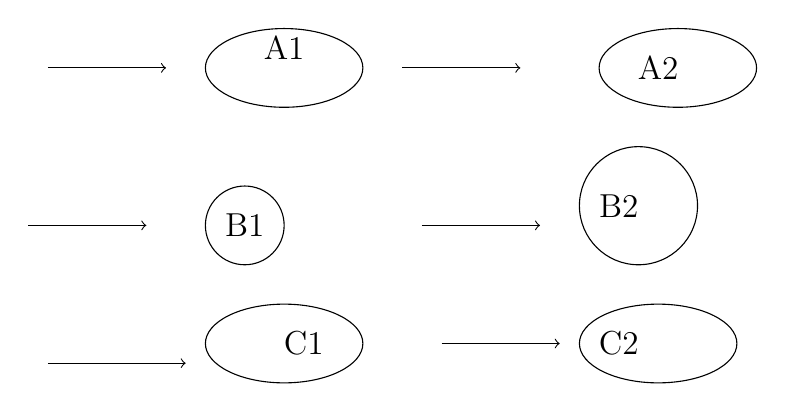
\begin{tikzpicture}
    \tikzstyle{every node}=[font=\large]
    
    % Row 1 (A1 to A2)
    \draw [->] (1.5,16.75) -- (3,16.75);
    \draw  (4.5,16.75) ellipse (1cm and 0.5cm);
    \draw [->] (6,16.75) -- (7.5,16.75);
    \draw  (9.5,16.75) ellipse (1cm and 0.5cm);
    \node at (4.5,17) {A1};
    \node at (9.25,16.75) {A2};

    % Row 2 (B1 to B2)
    \draw [->] (1.25,14.75) -- (2.75,14.75);
    \draw [->] (6.25,14.75) -- (7.75,14.75);
    \draw  (4,14.75) circle (0.5cm);
    \draw  (9,15) circle (0.75cm);
    \node at (4,14.75) {B1};
    \node at (8.75,15) {B2};

    % Row 3 (C1 to (1.5,13) -- (3.25,13);
    \draw [->] (1.5,13) -- (3.25,13);
    \draw  (4.5,13.25) ellipse (1cm and 0.5cm);
    \draw [->] (6.5,13.25) -- (8,13.25);
    \draw  (9.25,13.25) ellipse (1cm and 0.5cm);
    \node at (4.75,13.25) {C1};
    \node at (8.75,13.25) {C2};

\end{tikzpicture}
\begin{enumerate}
    \item 1,3 \& 6
    \item 2,3 \& 6
    \item 1,3 \&5
    \item 1,4 \& 6
\end{enumerate}
\bigskip
\item Consider 2-D, steady, incompressible, fully developed flow of viscous, Newtonian fluid through two stationary parallel plates, in Cartesian co-ordinate $\brak{x,y,z}$ system. Assume plates are very long in x-direction, wide in z-direction $\brak{\text{also there is no variation of velocity in z direction}}$ and distance between them is 2h. The velocity in such a channel is given as $\mathbf{U}=\mathbf{U}_{max}\brak{a-\frac{y^2}{h^2}}$ The origin y =0 is located at the center between the plates. If h = 48 mm and $\mathbf{U_{max}=100mm/s}$ difference between values of stream functions passing through y = 0 and y = $\frac{h}{2}$ is $\cdots$ mm$^2$/s.
\bigskip
\item A pump is used to deliver water to an overhead tank at a flow rate of $\mathbf{Q}=4\times 10^{-3}m^3/s$. The pump adds 1.6 kW to water. If the density of water is 1000 kg/$m^3$ and acceleration due to gravity is 10 $m/s^2$, the pump head added to the flow is  m.
\bigskip
\item Water is discharged at atmospheric pressure from a large reservoir through a long pipe of diameter d and length L. The height of the free surface of the reservoir from the discharge point is h meters. The Darcy's friction factor of the pipe is 0.002. Neglect the velocity inside the reservoir as the reservoir is very large. Given, L = 20m, d = 40mm, density of water = 1000kg/m$^3$ and flow rate is $\mathbf{Q}=4\pi \times 10^{-3} m^3/s$. Assume gravitational acceleration, g = 10 m/s$^2$. The value of h is $\cdots$
\bigskip
\item Energy Dispersive Spectroscopy $\brak{\text{EDS}}$ in a typical scanning electron microscope enables elemental identification by collecting and examining which of the following:
\begin{enumerate}
    \item Secondary electrons from the sample
     \item Back scattered electrons from the sample
    \item Characteristic X-rays from the sample
    \item  Diffraction pattern from the sample
\end{enumerate}
\bigskip
\item Which of the following rotational symmetry is forbidden in a perfectly periodic 3-dimensional lattice?
\begin{enumerate}
    \item 1-fold
    \item 3-fold
    \item 5-fold
    \item 6-fold
\end{enumerate}
\bigskip
\item Which of the following thermodynamic properties shows a discontinuity during a second-order phase transition?
\begin{enumerate}
    \item volume
    \item Enthalpy
    \item Entropy
    \item Heat capacity
\end{enumerate}
\bigskip
\item Cross slip is easily promoted in metals having
\begin{enumerate}
    \item a low stacking fault energy.
    \item a low grain boundary energy.
    \item a high stacking fault energy.
    \item a high grain boundary energy.
\end{enumerate}
\bigskip
\item For a typical metal at room temperature and atmospheric pressure, the Fermi energy is defined as the energy level for which the probability of occupancy is:
\begin{enumerate}
    \item 0
    \item 0.25
    \item 0.5
    \item 1
\end{enumerate}
\bigskip
\item Number of elements in a tensor of rank 4 is $\cdots$
\bigskip
\item Which one of the following effects is the working principle of a thermocouple?
\begin{enumerate}
    \item Thomson
    \item seebeck
    \item peltier
    \item Meissner
\end{enumerate}
\bigskip
\item At equilibrium, the maximum number of phases that can coexist in a ternary system at constant pressure is $\cdots$
\bigskip
\item Defect-free single crystal alumina $\brak{\text{sapphire}}$ is
\begin{enumerate}
    \item opaque and white
    \item transparent.
    \item translucent.
    \item opaque and black.
\end{enumerate}

